\section[Phylogenetic Clustering (Phyloclustering)]{Phylogenetic Clustering (Phyloclustering)}
\label{sec:phyloclustering}
\addcontentsline{toc}{section}{\thesection. Phylogenetic Clustering (Phyloclustering)}


Phylogenetic clustering (Phyloclustering) is a model-based
approach based on evolution theories to determine population
structures in molecular level.
Let $\vect{X} = (x_{nl})_{N\times L}$ be the data matrix containing
$N$ sequences observed of $L$ sites where $n = 1, \ldots, N$ and
$l = 1, \ldots, L$. Denote the sequence
$\vect{x}_n = (x_{n1}, \ldots, x_{nL}) \in \mathfrak{X}$ and
$x_{nl} \in \mathcal{S}$ where
$\mathfrak{X}$ contains all possible sequences and
$\mathcal{S}$ contains bases, e.g. $\mathcal{S} = \{\A, \G, \C, \T\}$
for nucleotide sequences.

A finite mixture distribution for model-based clusterings is
\begin{equation*}
f(\vect{x}_n | \vect{\eta}, \vect{\Theta}) =
\sum_{k = 1}^K \eta_k f_k(\vect{x}_n | \Theta_k)
\end{equation*}
where $f_k()$ is the density for $k$th component,
$\vect{\eta} = \{\eta_1, \ldots, \eta_K\}$ is the mixture proportion
summing to one, and
$\vect{\Theta} = \{\Theta_1,\ldots,\Theta_K\}$ contains parameters for
components.  By the Continuous Time Markov Chain theory,
$f_k()$ is modeled as transition probability
$p_{\vect{\mu}_k,\vect{x}_n}(t)$ of mutation process \citep{Felsenstein2004}.
A sequence $\vect{x}_n$ evolves from
a representative
$\vect{\mu}_k = (\mu_{k1}, \ldots, \mu_{kL}) \in \mathfrak{X}$
dominating the $k$th cluster where $\mu_{kl} \in \mathcal{S}$,
and process evolves with parameters $\vect{Q}_k$ in time $t_k$
which are allowed to differ, so that
$\Theta_k = \{\vect{\mu}_k, \vect{Q}_k, t_k\}$,
and the transition probability matrix can be computed by
$\mathbb{P}(t_k) = e^{\vect{Q}_k t_k}$ fot constructing likelihood functions.
This model can be solved by EM algorithms \citep{Dempster1977}, sequences can
be classified by the maximum posterior probabilities, and the number of
clusters can be assessed by bootstrapping \citep{Maitra2010}.

Usually, the $\vect{\mu}_k$'s are different with each other and
represent the central sequences of subpopulations.
The major evolution models used in $Q_k$ for nucleotide sequences supported in
the \pkg{phyclust} include \code{JC69} \citep{Jukes1969},
\code{K80} \citep{Kimura1980},
and \code{HKY85} \citep{Hasegawa1985}
which are indicated in \code{.substitution}.
I use an identifier (\code{.identifer}) to indicate possible combinations
of models for $\vect{Q}_k$ and $t_k$ and list in the
Table~\ref{tab:identifier}.
\begin{table}[h]
\begin{center}
\caption{Combinations of Models}
\begin{tabular}{ccc} \hline\hline
Identifier & $\vect{Q}$ & $t$ \\ \hline
\code{EE}  & $\vect{Q}_1 = \vect{Q}_2 = \cdots = \vect{Q}_K$
           & $t_1 = t_2 = \cdots = t_K$ \\
\code{EV}  & $\vect{Q}_1 = \vect{Q}_2 = \cdots = \vect{Q}_K$
           & $t_1 \neq t_2 \neq \cdots \neq t_K$ \\
\code{VE}  & $\vect{Q}_1 \neq \vect{Q}_2 \cdots \neq \vect{Q}_K$
           & $t_1 = t_2 = \cdots = t_K$ \\
\code{VV}  & $\vect{Q}_1 \neq \vect{Q}_2 \neq \cdots \neq \vect{Q}_K$
           & $t_1 \neq t_2 \neq \cdots \neq t_K$ \\
\hline\hline
\end{tabular}
\label{tab:identifier}
\end{center}
\end{table}

Note that there is an evolution distance model \code{.edist.model} that
I use to indicate the model for computing distance of paired sequences,
and they may differ to \code{.substitution}.
There are more options in the \pkg{ape} package \citep{Paradis2004}.

The \code{.show.option()} function will list all options
available in the \pkg{phyclust} package as the following.
These options can be used in the \code{.EMControl()} function
to generate a template for the \code{phyclust()} function.
\begin{Code}
> .show.option()
boundary method: ADJUST, IGNORE
code type: NUCLEOTIDE, SNP
edist model: D_JC69, D_K80, D_HAMMING
em method: EM, ECM, AECM
identifier: EE, EV, VE, VV
init method: randomMu, NJ, randomNJ, PAM, K-Medoids, manualMu
init procedure: exhaustEM, emEM, RndEM, RndpEM
standard code: 
     nid code code.l
[1,]   0    A      a
[2,]   1    G      g
[3,]   2    C      c
[4,]   3    T      t
[5,]   4    -      -
     sid code
[1,]   0    1
[2,]   1    2
[3,]   2    -
substitution model: 
          model  code.type
 [1,]      JC69 NUCLEOTIDE
 [2,]       K80 NUCLEOTIDE
 [3,]       F81 NUCLEOTIDE
 [4,]     HKY85 NUCLEOTIDE
 [5,]  SNP_JC69        SNP
 [6,]   SNP_F81        SNP
 [7,]     E_F81 NUCLEOTIDE
 [8,]   E_HKY85 NUCLEOTIDE
 [9,] E_SNP_F81        SNP
\end{Code}

All options will be explained in the help page and the short explanation
will be given on our website.
Some options may perform better than others in different situations.
For EM algorithms, several initializations are necessary to obtain
a better result, see the Section~\ref{sec:emcontrol}.




\subsection[Illustrate data]{Illustrate data}
\label{sec:illustrate}
\addcontentsline{toc}{subsection}{\thesubsection. Illustrate data}

The toy dataset has 100 nucleotide sequences and 200 sites in 4 clusters
where the ancestral tree height 0.15 and the descendant tree height 0.09,
and sequences are evolved by a HKY85 model \citep{Hasegawa1985}.
The 4 clusters are isolated
in groups, but they also carry common information about their ancestral
sequences and differ with each other at some mutated sites.

The following code shows a plot in the Figure~\ref{fig:toydots}
to illustrate the sequences.
Each row represents a sequence in the order of the dataset,
the matrix \code{X}, and each column represents a site.
Assume the first sequence in the first cluster of the toy dataset
is the common/consensus sequence.
The dashed lines split the clusters.
The row fully drawn with colors is the common sequence,
and colors represent 4 different nucleotides.
Other rows are drawn the mutations indicated by colors
comparing to the common sequence.
The bottom row indicates the segregating sites which are sites containing
at least one mutations with the origin dots.
\begin{Code}
> seq.data.toy
code.type: NUCLEOTIDE, n.seq: 100, seq.len: 200.
> X <- seq.data.toy$org
> X.class <- as.numeric(gsub(".*-(.)", "\\1", seq.data.toy$seqname))
> plotdots(X, X.class)
\end{Code}
\begin{figure}[h]
\begin{center}
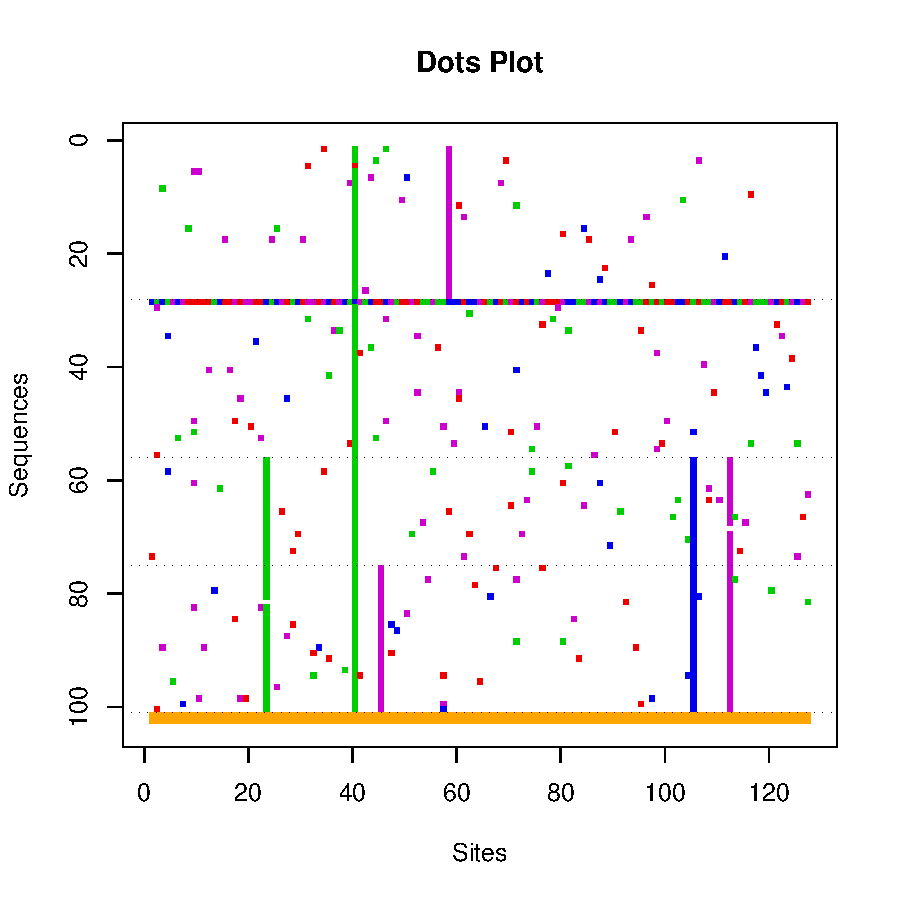
\includegraphics[width=5.0in]{./phyclust-graph/toydots}
\caption{A dot plot for the toy dataset.}
\label{fig:toydots}
\end{center}
\end{figure}

The following code provides a plot in the Figure~\ref{fig:toyhist}
to show the number of mutations by comparing all sequences to
the common sequence. The top plot is for the whole dataset,
the second to the bottom plots are for the sequences in
the first to the fourth clusters indicating by colors.
\begin{Code}
> plothist(X, X.class)
\end{Code}
\begin{figure}[h]
\begin{center}
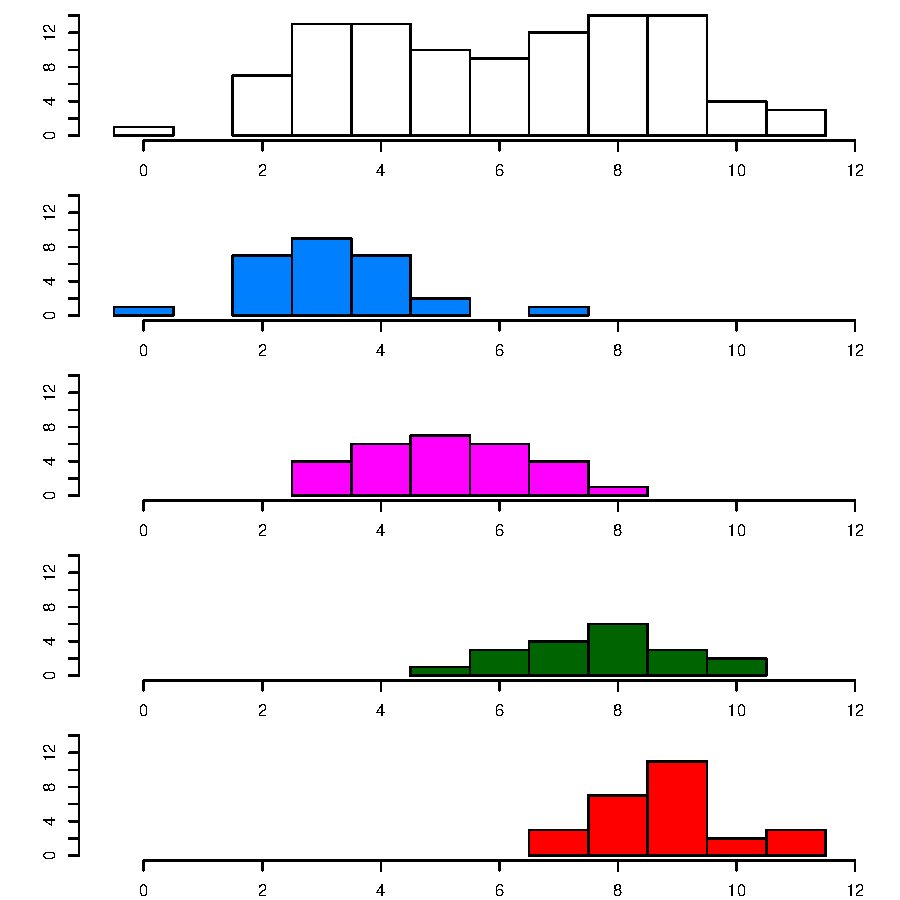
\includegraphics[width=5.0in]{./phyclust-graph/toyhist}
\caption{A histogram plot for the toy dataset.}
\label{fig:toyhist}
\end{center}
\end{figure}

The following code shows a plot in the Firgure~\ref{fig:toynj}
to illustrate the distance method which gives a rough structure
of dataset.
The \code{phyclust.edist()} function takes in a data
matrix \code{X}, compute and return pairwise distances for all sequences
where \code{.edist.model[3]} is \code{D_HAMMING} and the HAMMING distance
is used as a distance measure.
I apply a neighbor-joining method to build a tree based
on the distance matrix. The colors drawn on the leaf branches indicate
the clusters.
\begin{Code}
> (ret <- phyclust.edist(X, edist.model = .edist.model[3]))
Class 'dist'  atomic [1:4950] 4 3 4 7 2 4 5 5 8 2 ...
  ..- attr(*, "Size")= int 100
  ..- attr(*, "Diag")= logi FALSE
  ..- attr(*, "Upper")= logi FALSE
  ..- attr(*, "method")= chr "D_HAMMING"
> (ret.tree <- nj(ret))

Phylogenetic tree with 100 tips and 98 internal nodes.

Tip labels:
        1, 2, 3, 4, 5, 6, ...

Unrooted; includes branch lengths.
> plotnj(ret.tree, X.class = X.class)
\end{Code}
\begin{figure}[h]
\begin{center}
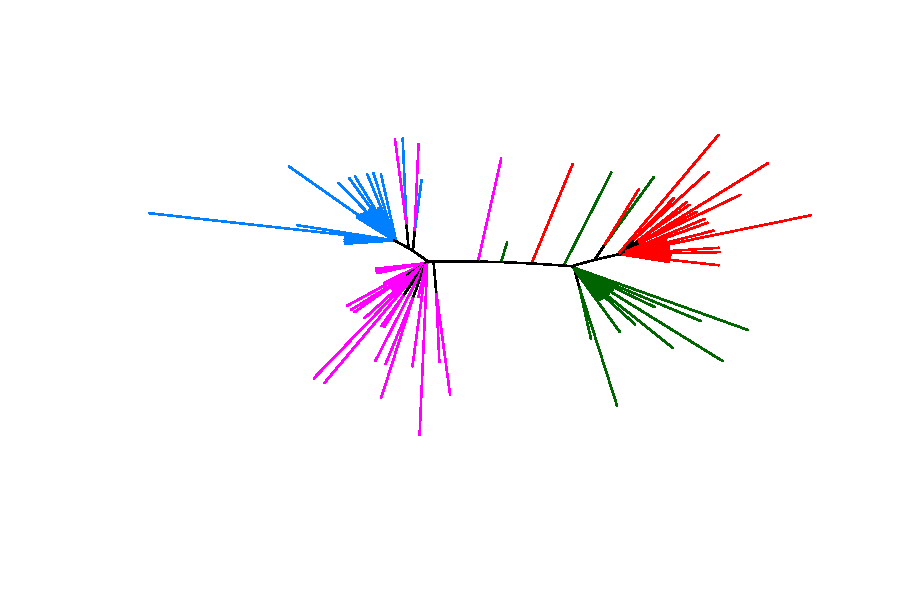
\includegraphics[width=5.0in]{./phyclust-graph/toynj}
\caption{A NJ tree for the toy dataset.}
\label{fig:toynj}
\end{center}
\end{figure}


\subsection[Use the phyclust() function]{Use the \code{phyclust()} function}
\label{sec:phyclust}
\addcontentsline{toc}{subsection}{\thesubsection. Use the \code{phyclust()} function}

I use the toy dataset to demonstrate the \code{phyclust()} function.
Basically, the \code{phyclust()} function takes in two required objects,
a data matrix \code{X} and the number of clusters \code{K}, then it
will fit a default model for \code{X} based on \code{EMC = .EMC}
which specifies models and optimizations. I will introduce this default
control \code{.EMC} and the function \code{.EMControl()} to generate it
in the Section~\ref{sec:emcontrol}.
In the following example, I fit a default model with 4 clusters to the
toy data.
\begin{Code}
> set.seed(1234)
> (ret.1 <- phyclust(X, 4))
Phyclust Results:
code type: NUCLEOTIDE, em method: EM, boundary method: ADJUST.
init procedure: exhaustEM, method: randomMu.
model substitution: JC69, distance: D_JC69.
iter: 37 3158 0, convergence: 0, check.param: 1.
eps: 4.851e-13, error: 0.
N.X.org: 100, N.X.unique: 87, L: 200, K: 4, p: 804, N.seg.site: 127.
logL: -1439, bic: 6581, aic: 4487, icl: 6588
identifier: EE
  Eta: 0.4360 0.01149 0.284 0.2700 
  Tt: 0.003325 
  n.class: 44 1 28 27
> RRand(ret.1$class.id, X.class)
   Rand adjRand  Eindex 
 0.9018  0.7653  0.1655
> class(ret.1)
[1] "phyclust"
\end{Code}

From the above reports, the default settings are used and
the result does not fit well (with a degenerated cluster, see \code{n.class})
due to the initialization problem. The initialization procedure
is \code{exhaustEM} and the initialization method is \code{randomMu},
so it randomly picks 4 sequences as the center of clusters and
run the EM algorithm to convergence. While the EM algorithms do not guarantee
to converge to global optimizations, more initializations should be
explored to seek a better solution efficiently.
The adjusted Rand index \citep{Hubert1985}, \code{adjRand}, is about 0.7653.
The \code{phyclust} function returns a list object with class
{\color{red} \code{phyclust}}
and it can be as an input of other functions such as the function
\code{bootstrap.star.trees.seq()} for bootstrapping.
in the Section~\ref{sec:msseqgenphyclust}.




\subsection[Use the .EMControl() function]{Use the \code{.EMControl()} function}
\label{sec:emcontrol}
\addcontentsline{toc}{subsection}{\thesubsection. Use the \code{.EMControl()} function}

The \code{.EMControl()} function provides a list object as the default
value for the \code{phyclust()} function. The internal object \code{.EMC}
is a template. Each element indicates a configuration for evolution models,
identifier, initialization, optimizations, and EM algorithms. See the help
page for details, and visit our website for examples.
\begin{Code}
> ?.EMControl
> ?.EMC
\end{Code}


You can either modify from the template \code{.EMC} or use the function
\code{.EMControl()} to generate a new control.
First, the following example modifies an object coping from the template.
It uses "emEM" as an initialization procedure, and
the result of \code{ret.2} has a higher likelihood value than that
of \code{ret.1}.
The adjusted Rand index is also 1 that the prediction has a perfect match
to the dataset.
\begin{Code}
> EMC.2 <- .EMC
> EMC.2$init.procedure <- .init.procedure[2]
> ### The same as
> ### EMC.2 <- EMControl(init.procedure = "emEM")
> set.seed(1234)
> (ret.2 <- phyclust(X, 4, EMC = EMC.2))
Phyclust Results:
code type: NUCLEOTIDE, em method: EM, boundary method: ADJUST.
init procedure: emEM, method: randomMu.
model substitution: JC69, distance: D_JC69.
iter: 103 8725 0, convergence: 0, check.param: 1.
eps: 2.753e-14, error: 0.
N.X.org: 100, N.X.unique: 87, L: 200, K: 4, p: 804, N.seg.site: 127.
logL: -1379, bic: 6461, aic: 4367, icl: 6469
identifier: EE
  Eta: 0.2700 0.1898 0.2801 0.2602 
  Tt: 0.003074 
  n.class: 27 19 28 26
> RRand(ret.2$class.id, X.class)
   Rand adjRand  Eindex 
 1.0000  1.0000  0.1209
\end{Code}

Second, the following use the function \code{.EMControl()} to generate a
new control that uses "RndEM" as an initialization procedure, and
fit a model with an "EV" identifier. An over fitted model can also cause
a degenerated cluster and usually needs more initializations to have a
better result.
From the output,
the \code{Eta} of the second cluster is smaller than others,
and the \code{Tt} gives an evolving time for sequences away from the ancestor
of the cluster, and the second cluster has a longer time than others.
This makes the second cluster is degenerated.
\begin{Code}
> EMC.3 <- .EMControl(init.procedure = "RndEM", identifier = "EV")
> ### The same as
> ### EMC.3 <- .EMC
> ### EMC.3$init.procedure <- .init.procedure[3]
> ### EMC.3$identifer <- .identifier[3]
> set.seed(1234)
> (ret.3 <- phyclust(X, 4, EMC = EMC.3))
Phyclust Results:
code type: NUCLEOTIDE, em method: EM, boundary method: ADJUST.
init procedure: RndEM, method: randomMu.
model substitution: JC69, distance: D_JC69.
iter: 104 51836 0, convergence: 0, check.param: 1.
eps: 4.278e-13, error: 0.
N.X.org: 100, N.X.unique: 87, L: 200, K: 4, p: 807, N.seg.site: 127.
logL: -1453, bic: 6621, aic: 4519, icl: 6627
identifier: EV
  Eta: 0.2696 0.01149 0.2844 0.4461 
  Tt: 0.002230 4.75 0.003663 0.003924 
  n.class: 27 0 28 45
> RRand(ret.3$class.id, X.class)
   Rand adjRand  Eindex 
 0.9002  0.7640  0.1698
\end{Code}

Note that an convenient function \code{find.best()} is useful to
search the best result based on the highest likelihood value by
repeatedly running on possible combinations
of the \code{.EMControl()} function. This function may also take
time to obtain a result.




\subsection[The ms+seqgen+phyclust approach]{The ms+seqgen+phyclust approach}
\label{sec:msseqgenphyclust}
\addcontentsline{toc}{subsection}{\thesubsection. The ms+seqgen+phyclust approach \vspace{-0.3cm}}

Usually, the assessment for a fitted model includes the number of clusters,
the evolution models, and the identifiers for clusters. All of these may
rely on information criteria, but it may not accurate and sometimes
it may give a wrong answer. A more elegant procedure is based on
the parameter bootstrap technique \citep{Maitra2010}.
The basic idea is
to bootstrap sequences by the functions \code{ms()} and \code{seqgen()}
and re-sample from a fitted model, a result of the \code{phyclust}
function.

The \code{bootstrap.star.trees.seq()} function implements this procedure
that it takes in a fitted model, \code{pcobj}, a list object with class
\code{phyclust} and utilizes the functions \code{ms()} and \code{seqgen()}
to re-sample new datasets. We can perform the same fitting method on
all new datasets to obtain an expected distribution of parameters,
and compared to the observed distribution obtained from the fitted model.

The following gives an example how to obtain a new datasets from a
model with 2 clusters based on the toy dataset.
The function \code{bootstrap.star.trees.seq()} returns a list object
contains two elements \code{trees} and \code{seq} for all clusters.
Combining \code{seq} and using the function \code{read.seqgen} can
read in the new dataset and save as a list object with class
\code{seq.data}.
\begin{Code}
> set.seed(1234)
> ret.4 <- phyclust(X, 2)
> ret.all <- bootstrap.star.trees.seq(ret.4)
> str(ret.all)
List of 2
 $ trees:List of 2
  ..$ :List of 5
  .. ..$ edge       : int [1:102, 1:2] 53 54 54 55 56 57 57 58 58 56 ...
  .. ..$ Nnode      : int 51
  .. ..$ tip.label  : chr [1:52] "42" "52" "27" "47" ...
  .. ..$ edge.length: num [1:102] 0.00000 0.00385 0.00000 0.00000 0.00000 ...
  .. ..$ n.tip      : int 52
  .. ..- attr(*, "class")= chr "phylo"
  ..$ :List of 5
  .. ..$ edge       : int [1:94, 1:2] 49 50 50 49 51 52 53 54 54 55 ...
  .. ..$ Nnode      : int 47
  .. ..$ tip.label  : chr [1:48] "16" "43" "10" "38" ...
  .. ..$ edge.length: num [1:94] 0.00000 0.00385 0.00385 0.00000 0.00000 ...
  .. ..$ n.tip      : int 48
  .. ..- attr(*, "class")= chr "phylo"
 $ seq  :List of 2
  ..$ :Class 'seqgen'  chr [1:53] " 52 200" "42        GAGATCTTGACCGCTTT ...
  ..$ :Class 'seqgen'  chr [1:49] " 48 200" "16        GAGATCTTGACCGCTTT ...
> toy.new <- c(paste(ret.4$N.X.org, ret.4$L, sep = " "),
+              ret.all$seq[[1]][-1], ret.all$seq[[2]][-1])
> ### Not necessary, but keep consistence.
> ### class(toy.new) <- "seqgen"
> (X.new <- read.seqgen(toy.new))
code.type: NUCLEOTIDE, n.seq: 100, seq.len: 200.
> (ret.5 <- phyclust(X, 2))
Phyclust Results:
code type: NUCLEOTIDE, em method: EM, boundary method: ADJUST.
init procedure: exhaustEM, method: randomMu.
model substitution: JC69, distance: D_JC69.
iter: 39 3035 0, convergence: 0, check.param: 1.
eps: 1.616e-12, error: 0.
N.X.org: 100, N.X.unique: 87, L: 200, K: 2, p: 402, N.seg.site: 127.
logL: -1571, bic: 4993, aic: 3946, icl: 4994
identifier: EE
  Eta: 0.4444 0.5556 
  Tt: 0.003846 
  n.class: 44 56
\end{Code}

